\chapter{Lec 18 - Machine Learning II}

\section{VC bound and SRM}
Consider a binary classification learning problem with:
\begin{itemize}
    \item Training set $S = \{(\textbf{x}_{1},y_{1}),...,(\textbf{x}_{n},y_{n})\}$.
    \item Hypothesis space $H = \{h_{\theta}(\textbf{x})\}$.
    \item Learning algorithm $L$, returning the hypothesis $g = h_{\theta}^{*}$ minimizing the empirical error on $S$, that is $g = argmin_{h \in H}error_{S}(h)$.
\end{itemize}
It is possible to derive \footnote{We will not see the derivation here.} an upper bound of the ideal error which is valid with probability $(1-\delta)$, $\delta$ being arbitrarily small, of the form:
\[error(g) \leq error_{S}(g) + F(\frac{VC(H)}{n},\sigma)\]
where $error(g)$ is the ideal error. The term $F(\frac{VC(H)}{n},\sigma)$ is called \textbf{VC-confidence} and it depends on:
\begin{itemize}
    \item The training set size $n$ (inversely).
    \item The VC-dimension of $H$, $VC(H)$ (proportionally).
    \item The confidence $\sigma$ (inversely).
\end{itemize}
As the VC-dimension grows, you usually observe that the empirical error decreases and that the VC confidence increases. So you can use the inductive principle \textbf{Structural Risk Minimization (SRM)} in order to minimize the right side of the confidence bound to get a tradeoff between the empirical error and the VC confidence.
\begin{center}
    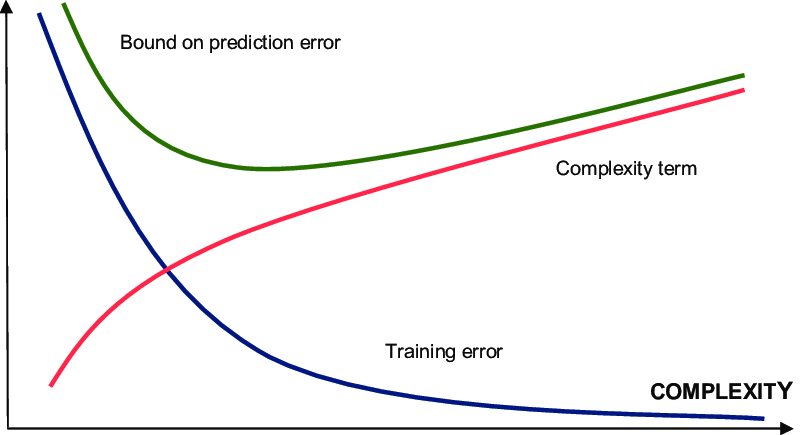
\includegraphics[scale=0.3]{images/Structural-risk-minimization-principle-Vapnik-1998.png}
\end{center}

\section{In Practice: how to use data}
The machine learning pipeline can be divided in two parts: the training phase and the testing phase. The first part involves:
\begin{enumerate}
    \item Analysis of the problem (Classification, Regression, ...)

    \item Collection, analysis and cleaning data

    \item Pre-processing and managing missing values

    \item Study of correlation between variables 

    \item Feature selection/weighting/learning

    \item Choice of the predictor and model selection
\end{enumerate}
Once the model is trained, we need to \textbf{test it} on new unseen data (not used during training).

\subsection{Model selection}
Model selection is the process used to compare different models and select the optimal one. In particular, model selection can be performed with respect to different values of the hyper-parameters of a fixed model.\newline\newline
There are several methods used to implement it. A first example can be the so called Hold-out procedure. The idea is to obtain a validation set (or hold-out set) $Va$ by splitting the training set $Tr$. Then, the fixed model is trained using examples in $Tr - Va$, trying different values of the hyper-parameters, and tested against the validation set. This procedure allows you to get an estimate of the error of the model on new unseen data.\newline\newline
Another approach for model selection (and evaluation) is the K-fold cross-validation:
\begin{enumerate}
    \item The training set is partitioned in $k$ disjointed validation sets $Va_{1},...,Va_{k}$. For each classifier $h_{1},...,h_{k}$, we apply the hold-out method on the $k$-th pair, that is, we train $h_{i}$ using examples in $Tr - Va_{i}$ and we test it against $V_{i}$. 

    \item Final error is obtained by individually computing the errors of $h_{1},...,h_{k}$ on the corresponding validation set and averaging the results.
\end{enumerate}
The above procedure is repeated for different values of the hyper-parameters and the predictor with the smallest final error is selected. The special case where $k = |Tr|$ (the validation sets are made of only one example) is called \textbf{leave-one-out} cross-validation.

\section{Artificial Neural Networks}
An Artificial Neural Network (ANN) is a system consisting of interconnected units that compute nonlinear (numerical) functions. The non linearity of the model is given by the activation functions. In fact, without them (linear activation) the result of the model, even if it’s very complex, would still be linear. ANNs consist of:
\begin{itemize}
    \item \textbf{input units}, which represent input variables;
    \item \textbf{output units}, which represent output variables;
    \item \textbf{hidden units} (if present), which represent internal variables that codify (after learning) correlations among input and desired output variables. Usually the output of hidden units is passed through a non-linear function called \textbf{activation function}. 
    \item adjustable \textbf{weights} which are associated to connections among units.
\end{itemize}
Thanks to the non-linear activation function, ANNs are able to exploit a more complex decision surface to solve tasks that a linear model would not be able to solve (e.g. XOR problem). Note that, in order to exploit gradient-based optimization, the activation function must be derivable.

\section{Gradient Descent for Feed-forward Networks}
The basic idea of the learning algorithm for ANNs consists in two phases:
\begin{itemize}
    \item \textbf{Forward phase:} for each example in the training set, present it to the network and compute the output.
    \item \textbf{Backward phase:} Back-propagate the committed error by computing the gradients of the cost function with respect to the network's weights. 
\end{itemize}
\textbf{Backpropagation} is the algorithm used to \textbf{compute the gradient} of the loss function with respect to each parameter. The information from the cost function flows backward to compute these gradients. Then, another algorithm performs learning using the gradients (e.g. stochastic gradient descent).\\\\
Let's define some terminology:
\begin{itemize}
    \item $d$ \textbf{input units}: $d$ input data size $\textbf{x} \equiv (x_{1},...,x_{d})$, $d + 1$ when including the bias in the weight vector $\textbf{x}^{'} \equiv (x_{0}, x_{1},...,x_{d})$

    \item $n_{H}$ \textbf{hidden units} (with output $\textbf{y} \equiv (y_{1},...,y_{n_{H}})$)

    \item $c$ \textbf{output units}: $\textbf{z} \equiv (z_{1},...,z_{c})$. The number of desired output is $\textbf{t} \equiv (t_{1},...,t_{c})$

    \item $w_{ji}$ weight from the $i$-th input unit to the $j$-th hidden unit ($w_{j}$ is the weight vector of the $j$-th hidden unit)

    \item $w_{kj}$ weight from the $j$-th hidden unit to the $k$-th output unit ($w_{k}$ is the weight vector of the $k$-th output unit)
\end{itemize}
Let's consider, for example, a Neural Network with just one hidden layer and \textbf{sigmoid activation functions}. We need to minimize an error function $E[\textbf{w}]$ that can be defined as follows:
\[E[\textbf{w}] = \frac{1}{2cN}\sum_{s=1}^{N}\sum_{k=1}^{c}(t_{k}^{(s)} - z_{k}^{(s)})^{2}\]
We need to first compute the gradient for the weights of both output and hidden units.
\begin{itemize}
    \item \textbf{Gradient of the weights of an output unit:}
    \[\frac{\partial E}{\partial w_{\hat{k}\hat{j}}} = - \frac{1}{cN}\sum_{s=1}^{N}(t_{\hat{k}}^{(s)} - z_{\hat{k}}^{(s)} )z_{\hat{k}}(1 - z_{\hat{k}})y_{\hat{j}}^{(s)}\]
    where $y_{\hat{j}}^{(s)}$ is the output of the $\hat{j}$-th hidden unit.
    
    \item \textbf{Gradient of the weights of a hidden unit:}
    \[\frac{\partial E}{\partial w_{\hat{j}\hat{i}}} = - \frac{1}{cN}\sum_{s=1}^{N}y_{\hat{j}}^{(s)}(1 - y_{\hat{j}}^{(s)})x_{\hat{i}}^{(s)}\sum_{k=1}^{c}(t_{\hat{k}}^{(s)} - z_{\hat{k}}^{(s)} )z_{\hat{k}}(1 - z_{\hat{k}})w_{k\hat{j}}\]
\end{itemize}

\textbf{Back-propagation (stochastic)}
\begin{enumerate}
    \item Initialize all weights with small random values (e.g. between -0.5 and +0.5)
    \item Until the termination condition is satisfied:
    \begin{enumerate}
        \item For each $(\textbf{x},\textbf{t}) \in S$:
        \begin{enumerate}
            \item Present $\textbf{x}$ to the net and compute the vectors $\textbf{y}$ and $\textbf{z}$
            \item For each output unit $k$:
            \[\delta_{k} = z_{k}(1 - z_{k})(t_{k} - z_{k})\]
            \[\Delta w_{kj} = \delta_{k}y_{j}\]

            \item For each hidden unit $j$:
            \[\delta_{j} = y_{j}(1 - y_{j})\sum_{k=1}^{c}w_{kj}\delta_{k}\]
            \[\Delta w_{ji} = \delta_{j}x_{i}\]

            \item Update all weights:
            \[w_{sq} \leftarrow w_{sq} + \eta \Delta w_{sq}\]
        \end{enumerate}
    \end{enumerate}
\end{enumerate}
Note that this algorithm works only for a network with one hidden layer, but can be easily extended. In fact, the algorithm computes the error term $\delta$ for each unit of each layer, and then it multiplies this error term for the input of the unit.

\section{Deep Learning}
Deep neural networks are ANNs with several hidden layers between input and output units. It is convenient to use more than one hidden layer in a neural network because a multi-layer neural network can learn high-level non-linear representations of the input data which may improve the effectiveness of the model. Basically, instead of providing to the model hand-designed features, we let the model to automatically learn abstract representations of data and use them to perform a specific task. Furthermore, deep networks seem to generalize better.
